\documentclass{beamer}
%\usepackage{graphicx} % Already loaded by beamer!
\usepackage{multicol}
\hypersetup{colorlinks,linkcolor=blue,urlcolor=cyan}


\title{Introduction to MATLAB}
\date{} % Suppress date

\beamertemplatenavigationsymbolsempty % Suppress navigation symbols
\begin{document}

\begin{frame}
\titlepage
\end{frame}

\section{Overview}
\begin{frame}{Overview}
	\begin{itemize}
		\item The purpose of this resource is to give a very basic introduction to MATLAB
		\item If you have no prior experience with MATLAB or computer programming, it's probably best to work through the slides in order
		\item Open MATLAB on your computer and wherever an example is given, try it for yourself in MATLAB
		\item If you have some prior MATLAB experience you may find it more useful to skip to specific sections of interest
		\item There are some \href{http://wiki.rac.manchester.ac.uk/community/MATLAB/IntroExercises}{exercises} with \href{http://wiki.rac.manchester.ac.uk/community/MATLAB/IntroSolutions}{solutions} which accompany this course, to help you solidify your understanding
	\end{itemize}
\end{frame}

\begin{frame}{Course outline}
	\begin{multicols}{2}
		\tableofcontents
	\end{multicols}	
\end{frame}

\section{Before you get started}
\begin{frame}{Before you get started}{Licence restrictions, installation instructions, considerate behaviour}
	\begin{itemize}
		\item Check the \href{https://www.applications.itservices.manchester.ac.uk/show_product.php?id=98&tab=licensing}{IT Services website} for licence restrictions, and other useful information organised by tabs...
		\item ...for example,  \href{https://www.applications.itservices.manchester.ac.uk/show_product.php?id=98&tab=install}{installation instructions} (if you use a managed desktop, see \href{http://www.itservices.manchester.ac.uk/our-services/desktop/your-desktop/windows7/applications/}{requesting a new application} instead)
		\item Ensure connection to University network licence i.e. connect to campus local-area network or \href{http://www.itservices.manchester.ac.uk/our-services/my-it/vpn/}{VPN} (staff only)
		\item The licence supports 616 concurrent research users (and generally fewer licences for MATLAB's toolboxes), so please:
		\begin{itemize}
			\item Don't leave MATLAB running unnecessarily
			\item Don't open MATLAB on multiple hardware
%			\item Create stand-alone executables  if running long calculations - use the MATLAB \texttt{mcc} compiler % This is a fair point, but probably unnecessary for an intro course. Mention in the Programming in MATLAB course instead.
		\end{itemize}
	\end{itemize}
\end{frame}

\section{The MATLAB desktop}
\subsection{Sub-windows}
\frame{
	\frametitle{MATLAB desktop windows}
	\begin{itemize}
		\item MATLAB has several movable sub-windows: current folder, command window (for entering commands), workspace (shows current variables).	
		\item To get back to the default layout:
		
		Home tab $\rightarrow$ Environment section $\rightarrow$ Layout button $\rightarrow$ Default
	\end{itemize}
	
	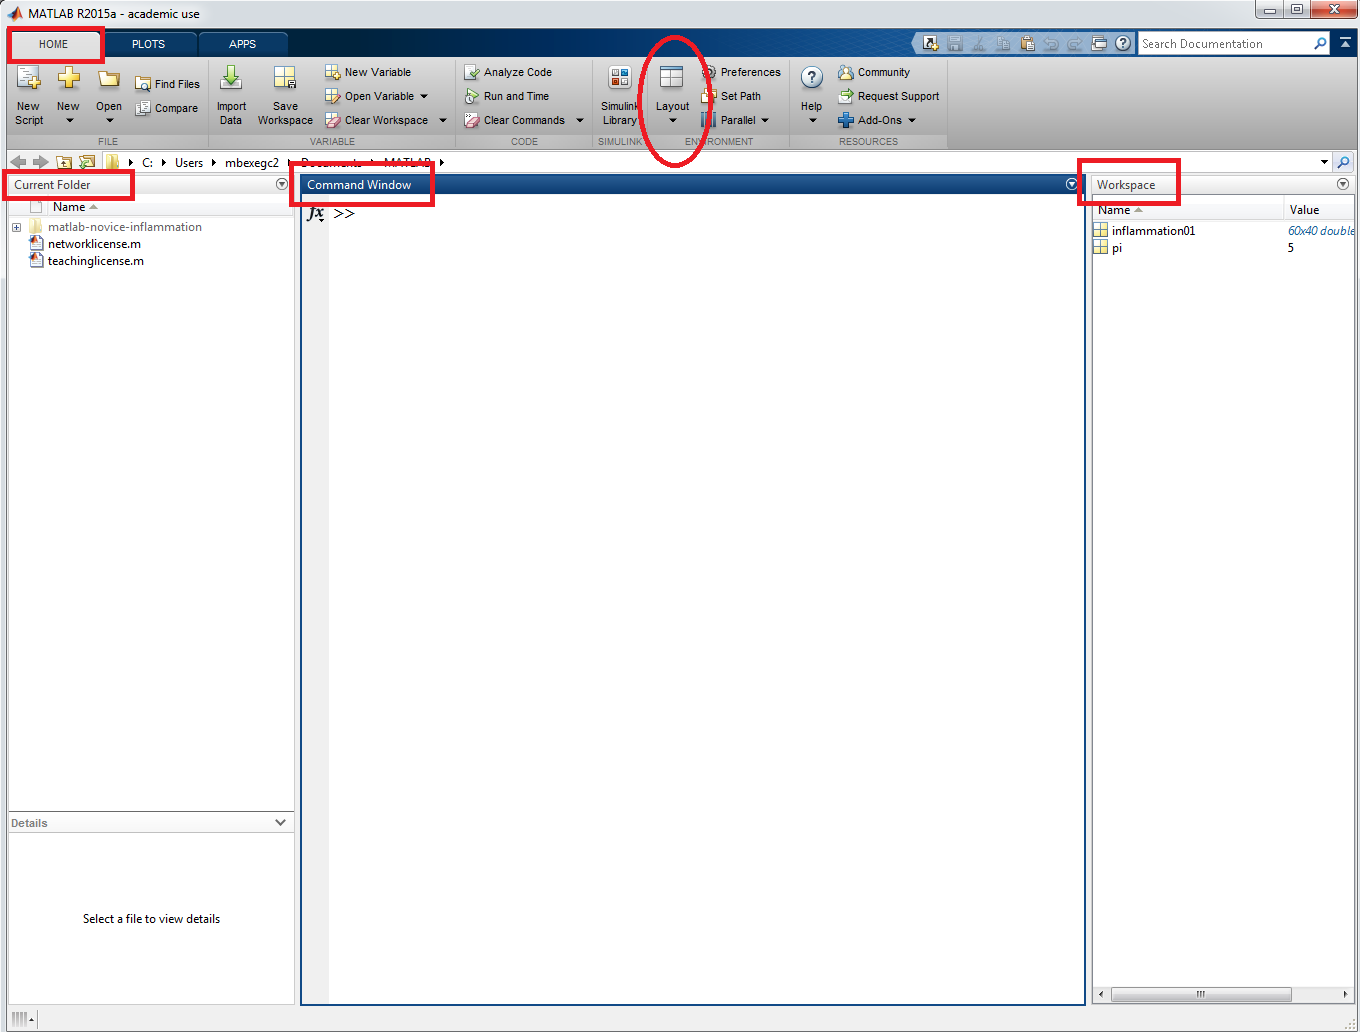
\includegraphics[width=\textwidth,trim={0 15cm 0 0},clip]{layout}
	\label{fig:layout}
	}
\subsection{Search path}
\frame{\frametitle{Setting the search path}
	\label{sec:path}
	\begin{itemize}
		\item MATLAB uses an internal variable called the path, which it uses when searching for files. It already knows where the MATLAB libraries are, but in order to find \textit{your} files (data files, MATLAB scripts that you have written etc), you will need to set the path.
		\item The current folder is shown in the red box below, and you can change the current folder by clicking on the button shown by the purple arrow. Files in this folder are now visible to MATLAB.
	\end{itemize}
	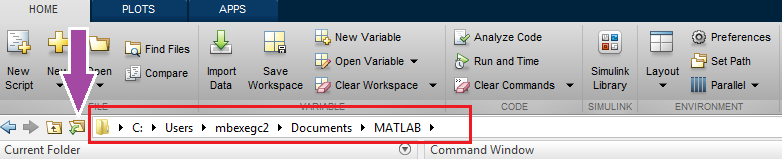
\includegraphics[width=\textwidth]{set_path}
	}
	
\subsection{The command window}		
\frame{\frametitle{The command window}
	\begin{itemize}
		\item This allows you to use MATLAB interactively, by typing commands at the prompt ($>>$ )
		\item After typing commands (alternatively, cut and paste), press \textbf{enter/return} key for MATLAB to run your command(s)
		\item This requires you to follow the rules of the MATLAB programming language
		\item If you enter an invalid command (e.g. typos) MATLAB will return an error
		\item The error may contain important information to help fix the problem (see example below)
	\end{itemize}
	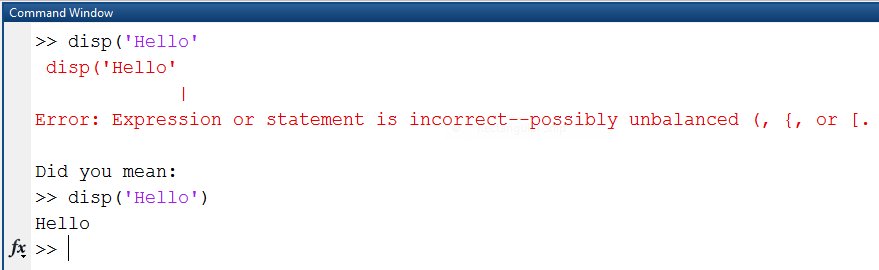
\includegraphics[width=\textwidth]{error_message}
}

\subsection{MATLAB documentation}
\frame{\frametitle{MATLAB help and documentation}
	\label{sec:matlab_help}
	\begin{itemize}
		\item MATLAB has very good help pages, which include example code
		\item To start help, click on the \textbf{help} button on the \texttt{home} tab or enter \texttt{doc} at the prompt ($>>$)
		
		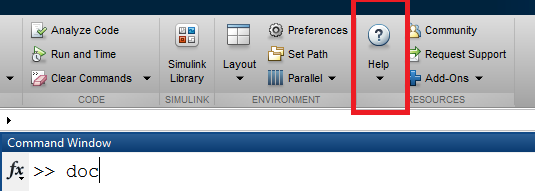
\includegraphics[width=\textwidth]{doc_help}
		
	\end{itemize}
}
\frame{

	\begin{itemize}
		\item For help with specific functions (e.g. plot), enter \texttt{doc plot} at the prompt to see the help pages or \texttt{help plot} to get information at the prompt
		\item Copy and paste MATLAB example code at the prompt to run
			
		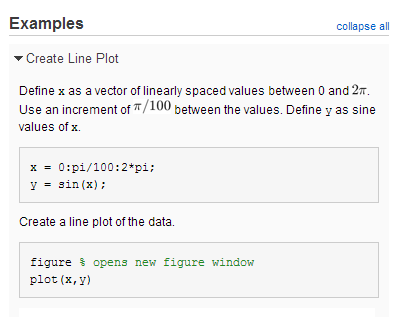
\includegraphics[width=.48\textwidth]{doc_plot}
		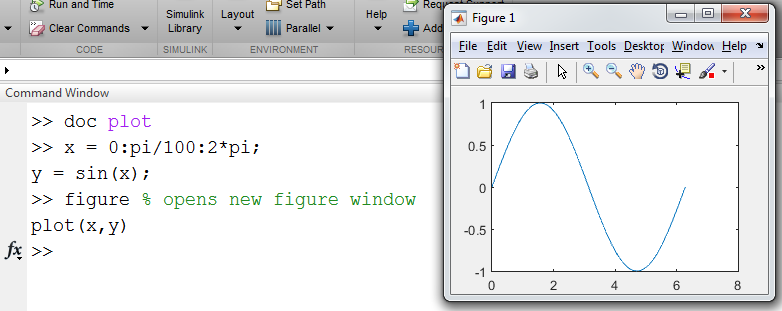
\includegraphics[width=0.48\textwidth]{plot_example}
	\end{itemize}	
}


\section{Variables}
\subsection{Creating variables}
\frame{
\frametitle{Creating variables}
	\begin{itemize}
		\item A variable allows us to assign data to a variable name
		\item To assign data to a variable, use the equals sign, =
		\item MATLAB first evaluates whatever is to the right of = , and then assigns this value to the variable
		\item To assign the result of 10 + 1 to a variable \texttt{var1}
		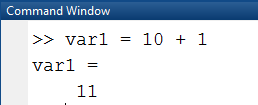
\includegraphics[width=0.5\linewidth]{assignment1}
		\item To assign the result of var1 - 3 to a new variable \texttt{var2}
		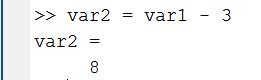
\includegraphics[width=0.5\linewidth]{assignment2}		
	\end{itemize}
}
\subsection{Reassigning variables}
\frame{\frametitle{Reassigning (overwriting) variables}
	\begin{itemize}
		\item To reassign our variable \texttt{var2} to be the cosine of zero
		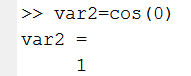
\includegraphics[width=0.5\linewidth]{reassign1}
		\item To add one to our variable \texttt{var2} (remembering that MATLAB first evaluates what is to the right of the  = , then assigns this value to the variable \texttt{var2} on the left)
		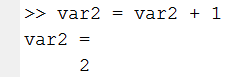
\includegraphics[width=0.5\linewidth]{reassign2}
	\end{itemize}
	}

\subsection{Variable names}
\frame{\frametitle{Variable names}
	\begin{itemize}
		\item These can contain letters, underscore and numbers
		\item They are case sensitive
		\item They must start with a letter
		\item namelengthmax returns maximum length (63 characters in MATLAB R2015a)
		\item Advice
		\begin{itemize}
			\item Choose descriptive names that aid understanding how the code works
			\item Don’t be afraid of long names if it makes code more readable e.g. \texttt{number\textunderscore of\textunderscore samples, BeamIntensity} 
		\end{itemize}
	\end{itemize}
	}

\frame{\frametitle{A warning about variable names}
	\label{sec:variable_names_warning}
	\begin{itemize}
		\item MATLAB will let you create variables with the same name as built in MATLAB variables and functions
		\item This hides the default MATLAB behaviour and therefore should be avoided
		\item MATLAB will not warn you if you do this
	\end{itemize}
	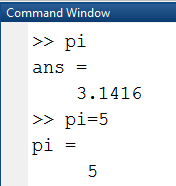
\includegraphics{variable_name_clash}
}

\frame{\frametitle{Working with variables}
	\begin{itemize}
		\item To list all variables in current workspace enter \texttt{who} or \texttt{whos}
		\item Variables are shown in the \texttt{Workspace} window - double click on them to view
		\item \texttt{clear} removes all variables, \texttt{clear variable1} removes \texttt{variable1} only
		\item Use \texttt{save} and \texttt{load} to save variables to/ load from files (by default MATLAB saves binary data files, which guarantees no loss of accuracy and is quicker than human-readable text)
		\item See MATLAB Help pages for more information ($>>$ \texttt{doc save; doc load})
	\end{itemize}
	}

\section{Arithmetic operators}
\frame{\frametitle{Arithmetic operators}
	\begin{itemize}
		\item MATLAB has the usual arithmetic operators 
		\begin{itemize}
			\item $+$ addition
			\item $-$ subtraction
			\item $*$ multiplication
			\item $/$ division
			\item $\hat{}$ exponentiation (e.g. 2.3 $\hat{}$ 5 = $2.3^5$)
		\end{itemize}
		\item Caution: for arrays * / and $\hat{}$ perform matrix operations
		\item For scalars, the above operators behave as expected
		\item See slide \ref{sec:matrix_operators} for more information
	\end{itemize}
	}

\section{Importing data}
\frame{\frametitle{Importing data}
	\begin{columns}
		\begin{column}{0.48\linewidth}
			\begin{itemize}
				\item Often you will want to import data from a file – e.g. comma separated values, Excel spreadsheets etc
				\item Note: some options for importing Excel spreadsheets require Excel to be
				installed – read the MATLAB documentation
				\item A good starting point is the \texttt{Import Data} button (on the Home
				tab) – this can generate scripts to automate the importing of data
			\end{itemize}
		\end{column}
		
		\begin{column}{0.48\linewidth}
			\begin{itemize}
				\item Browse to a data file, then click on \texttt{Import Selection}
				\item You can use these scripts as templates to import other data files
				
				\vspace{2mm}			
				
				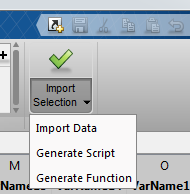
\includegraphics[width=0.8\linewidth]{data_import_generate_script}
			\end{itemize}
		\end{column}	
	\end{columns}
}

\section{Useful shortcuts and commands}
\frame{\frametitle{Useful shortcuts and commands}
	\begin{itemize}
		\item Up arrow key scrolls through previous commands (useful for fixing typos)
		\item Can type the first few characters at the prompt, then use up arrow to find commands which match the characters typed
		\item Tab auto-complete: type the first few letters of a command (e.g. function or variable) then press tab key to show completions
		
		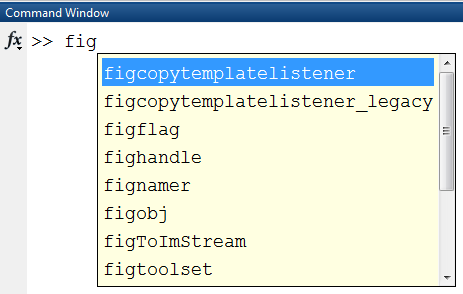
\includegraphics[width=0.7\linewidth]{tab_complete}
	\end{itemize}
	}

\frame{\frametitle{Working with folders}
	\begin{itemize}
		\item \texttt{pwd} prints current directory
		\item \texttt{ls} lists files in current directory (Note: the parent directory is represented by \texttt{..})
		\item \texttt{cd} changes directory 
		
		e.g. \texttt{cd ..} changes to the parent directory
		\item \texttt{mkdir }creates a new folder
		
		e.g. \texttt{mkdir newFolder}
		\item Search MATLAB Help for ``Manage Files and Folders''
		\item Alternatively use the \hyperlink{fig:layout}{\texttt{Current Folder }}Window
	\end{itemize}
}	
	
\section{Functions}
\frame{\frametitle{Functions}
	\begin{itemize}
		\item Most MATLAB functionality is accessed via functions
		\item To call (i.e. run) a function enter the function name
		\item Any data required by the function must be passed to the function as input arguments
		\item When the function finishes, values are passed back as output arguments
		\item Input and output arguments are sometimes optional
		\item In general MATLAB has very good documentation - read this to understand how to use MATLAB’s functions 
		
		(hint: $>>$ \texttt{function})
	\end{itemize}
}

\frame{\frametitle{Using functions}
	\framesubtitle{Brief overview - read the documentation for more detail}
	\begin{itemize}
		\item Input arguments in parentheses ( ) after the function name
		\item Output arguments in square brackets [ ] before the equals sign (brackets can be omitted for single output argument)
		\item Separate multiple arguments with commas
		
		e.g. \texttt{[out1, out2, out3] = func(in1, in2)}
		\item Some arguments may be optional (this will be described in MATLAB Help pages)
		\item MATLAB functions provide useful error messages - e.g.
		
		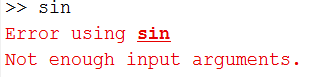
\includegraphics[width=0.5\linewidth]{function_error}
	\end{itemize}
}


\frame{\frametitle{MATLAB notation}\framesubtitle{The semicolon}
	\begin{itemize}
		\item By default MATLAB displays output after a command is run (e.g. Assigning variables, Calculations, Function calls)
		\item The semicolon suppresses this output, e.g.
		
		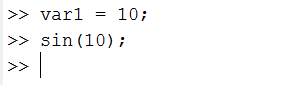
\includegraphics[scale=0.7]{semi-colon}
		\item This does not supress text printed to the screen from the command or function (e.g. via \texttt{disp} or \texttt{fprintf} - see MATLAB Help on \texttt{disp} and \texttt{fprintf})
	\end{itemize}
}


\frame{\frametitle{Some functions to start with}
	\begin{itemize}
		\item There are many built in MATLAB functions and operators
		\item Run the following commands to read about some key functions:
		\begin{itemize}
			\item \texttt{help ops} (lists operators)
			\item \texttt{doc operator precedence}
			\item \texttt{help elfun }(lists elementary maths functions)
			\item \texttt{help specfun }(lists specialised maths functions)
		\end{itemize}
	\end{itemize}
}

\frame{\frametitle{Toolboxes}
	\begin{itemize}
		\item Some MATLAB functions come in `add on' toolboxes
		\begin{itemize}
			\item Additional cost
			\item Possibly (very) limited number of licences
			\item Enter ver to see list of installed toolboxes
		\end{itemize}
		\item Just because a toolbox is installed doesn't mean there's a licence for it
		\item Each installed toolbox will have a top level entry in MATLAB Help
		\item Third party toolboxes can be added
		\begin{itemize}
			\item Some are free
			\item Advice: investigate quality before using (e.g. see \url{http://www.walkingrandomly.com/?p=2323})
		\end{itemize}
 
	\end{itemize}
}


\section{Data types}
\subsection{Some number types}
\frame{\frametitle{Some number types}
	\begin{itemize}
		\item Real numbers
		
		A rigorous definition is difficult, but basically not imaginary or complex. 
		They include whole numbers and fractions.

		e.g. $1, 2, 0 ,-1 ,3/5 , \pi, 34.23515, -2341, -234243.243242$
		
		\item Integers
		
		Whole numbers (i.e. a subset of real numbers)
		
		e.g. ...-6, -5, -4, -3, -2, -1 , 0, 1, 2, 3, 4, 5, 6...
		
		\item Imaginary numbers
		
		A number which when multiplied by itself gives a negative result
		
		e.g. $\sqrt{-1}$ is an imaginary number as $\sqrt{-1} \times \sqrt{-1} = -1$
		
		\item Complex numbers
		
		A number obtained by adding a real and imaginary number
		
		e.g. $\sqrt{−214.123} + 153$
	\end{itemize}
	}
\subsection{Numbers in MATLAB}
\begin{frame}{Numbers in MATLAB}{Double precision floating point}
	\begin{itemize}
		\item By default numbers are double precision floating point
		\begin{itemize}
			\item Double precision: 64 bits (binary digits) are used to store each value i.e. each bit represents either the value 1 or 0
			\item Accurate to around 16 significant decimal digits
			\item Most numbers represented by floating point are \textbf{approximations} to real numbers
			\item Conform to IEEE standard
			\item Includes Inf (infinity) and NaN (not a number)
		\end{itemize}
		\item So the following assigns a double precision floating point value to the variable var1
		$>>$ var1 = 10
		\item Floating point values are used to represent real numbers and double precision floating point numbers are very likely what you will use (most) in MATLAB
	\end{itemize}
\end{frame}

\begin{frame}{Floating point notation}
	\begin{itemize}
		\item \texttt{e} means times ten raised to the power of 
		
		e.g. 1e2 means $1 \times 10^{2}$ i.e. 100
		
		e.g. 1e-2 means $1 \times 10^{-2}$, i.e. $1/10^{2}$ or 0.01
		\item This allows us to represent very large and very small numbers e.g.
		
		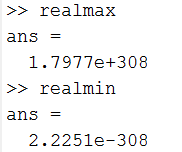
\includegraphics[scale=0.7]{realmax_realmin}
	\end{itemize} 
\end{frame}

\begin{frame}{Output precision}
	\begin{itemize}
		\item By default MATLAB displays numbers using up to 5 digits
		
		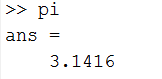
\includegraphics[scale=0.7]{pi_short}
		\item However, $\pi$ is a double precision value and has more precision than 5 digits
		\item We can change the format to show additional accuracy
		
		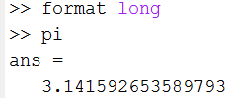
\includegraphics[scale=0.7]{pi_long}
		\item Look at the documentation for more information
	\end{itemize}
\end{frame}

\frame{\frametitle{Floating point versus real numbers}
	\begin{itemize}
		\item Floating point numbers are not real numbers
		
		Values are stored as \href{https://www.mathsisfun.com/binary-number-system.html}{binary numbers} (a series of ones and zeros). 
		General behaviour is close enough to reals for most purposes
		\item However it is very important to understand there are differences between real and floating point numbers. This is a topic for further reading e.g.
		The MATLAB Help page on ``Floating-Point Numbers'', and \href{https://docs.oracle.com/cd/E19957-01/806-3568/ncg_goldberg.html}{What Every Computer Scientist Should Know About Floating-Point Arithmetic}
		\item  For example: sine of $\pi$ is not zero in MATLAB
		
		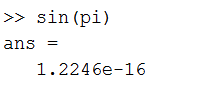
\includegraphics[scale=0.7]{floating_point_sin_pi}
		
	\end{itemize}
}

\frame{\frametitle{Floating point rounding}
	\begin{itemize}
		\item  In general not all real numbers can be represented exactly
		\item For example eps returns the distance between 1.0 and
		the next largest double-precision number
		– Real numbers between 1.0 and 1.0+eps can't be represented
		using MATLAB doubles
		– Values between 1.0 and 1.0 + eps will be rounded
		\item This introduces rounding errors
	\end{itemize}
}

\begin{frame}{Single precision floating point values}
	\begin{itemize}
		\item MATLAB also has single precision (32-bit) floating point numbers
		\begin{itemize}
			\item They require half as much memory to store
			\item They have less precision
			\item Around 8 significant decimal digits
		\end{itemize}
		\item They must be created explicitly e.g. using the \texttt{single }function
		 \item You probably won't use these, but it may be important to know they exist
		 
		 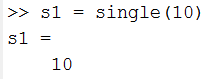
\includegraphics[scale=0.7]{single}
	\end{itemize}
\end{frame}

\begin{frame}{Complex numbers}
	\begin{itemize}
		\item in MATLAB \texttt{i} represents the square root of -1
		
		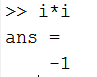
\includegraphics[scale=0.7]{i_squared}
		\item Complex arithmetic is fully supported e.g.
		
		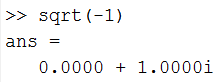
\includegraphics[scale=0.7]{sqrt-1}
		\item Enter \texttt{help complex} for more information
		\item Warning: do not use \texttt{i} as a variable name as this will hide MATLAB default behaviour (see slide \ref{sec:variable_names_warning})
	\end{itemize}
\end{frame}


\begin{frame}{Integers}
	\begin{itemize}
		\item MATLAB has various signed and unsigned integers
		\begin{itemize}
			\item Signed integers can take positive, zero and negative integer values
			\item Unsigned integers can only take positive and zero integer values
			\item There are 8, 16, 32 and 64 bit integers of each type (signed and unsigned)
		\end{itemize}
		\item Integers must be created explicitly
		\begin{itemize}
			\item For signed integers, use \texttt{int8, int16, int32, int64}
			\item For unsigned, use \texttt{uint8, uint16, uint32, uint64}
			\item e.g. to create an unsigned 8 bit integer
				$\texttt{>> var3 = uint8(24);}$
		\end{itemize}
		
		\item Integers with more bits require more memory
		\item More bits gives a wider range of possible values
	\end{itemize}
\end{frame}

\begin{frame}{Maximum and minimum numerical values}
	\begin{itemize}
		\item There are limits to the largest and smallest floating point values which can be represented
		\item There are limits to the most negative and most positive value for each integer type
		\item There are functions to give the value of these limits:
		
		\texttt{intmin, intmax, realmin, realmax}
		\item These limits can introduce errors to your computation e.g.
		
		\begin{itemize}
			\item Floating point results can differ significantly from equivalent real number calculations if very small values are involved
			\item Floating point calculations may return \texttt{Inf} or \texttt{-Inf}
			\item Integer results will be rounded to the maximum and minimum values for that type if out of range
		\end{itemize}
	\end{itemize}
\end{frame}

\subsection{Logical values}
\begin{frame}{Logical values}
	\begin{itemize}
		\item These represent the logical values \texttt{true} and \texttt{false}
		\item Values can be either \texttt{1 (true)} or \texttt{0 (false)}
		\item Assign using \texttt{true} or \texttt{false}
			
		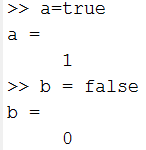
\includegraphics[scale=0.7]{true_false_assignment}
		\item Logical values are more often used when writing your own functions, but are also returned from some intrinsic MATLAB functions, so are useful to know about
	\end{itemize}
\end{frame}

\begin{frame}{More on data types}
	\begin{itemize}
		\item To find the type of the data use the \texttt{class} function - this returns the class of any MATLAB object e.g.
		
		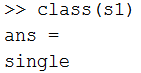
\includegraphics[scale=0.7]{return_class}
		\item Reminder: we can explicitly convert data types e.g.
		
		$\texttt{>> d1 = 10; \% d1 is double precision}$
		
		$\texttt{>> i1 = int8(d1); \% i1 is of class int8}$
		\item MATLAB automatically assigns the class for results involving multiple class types (e.g. multiplying a double and an integer)
		\item When undertaking calculations using multiple classes make sure you understand how MATLAB behaves (read the documentation or run tests)
	\end{itemize}
\end{frame}

\begin{frame}{Strings}
	\begin{itemize}
		\item Strings (i.e. text) are arrays of characters (We'll come to arrays later)
		\item They are of class \texttt{char}
		\item They are created using single quotes e.g.
		
		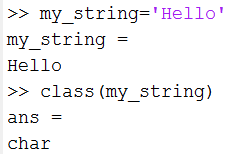
\includegraphics[scale=0.7]{string}
		\item Some MATLAB functions take strings as input arguments
	\end{itemize}
\end{frame}

\begin{frame}{Function handles}
	\begin{itemize}
		\item These allow a function to be to represented by a variable i.e. the variable can be used to execute the function
		\item The variable has the class \texttt{function\textunderscore handle}
		\item These can be created using the @ symbol e.g. create a function handle representing the sin function

		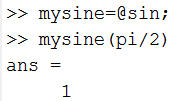
\includegraphics[scale=0.7]{sin_function_handle}
		\item We can use these to pass functions to other functions - e.g. try \texttt{ezplot(@sin)} or \texttt{ezplot(mysine)}
	\end{itemize}
\end{frame}

\begin{frame}{Cells}{Also known as Cell Arrays}
	\begin{itemize}
		\item These can contain multiple values of different data type
		\item Values are accessed using indices
		\item You may not need these, but they're useful to know about (search for \emph{Cell Arrays} in MATLAB documentation)
		\item They can be created using curly braces \{ \}
		\item These have the \texttt{cell} class
	\end{itemize}
\end{frame}

\begin{frame}{Structures}{Also known as Structure Arrays}
	\begin{itemize}
		\item These allow you to group related data of different types e.g.
		
		\vspace{2mm}
		
		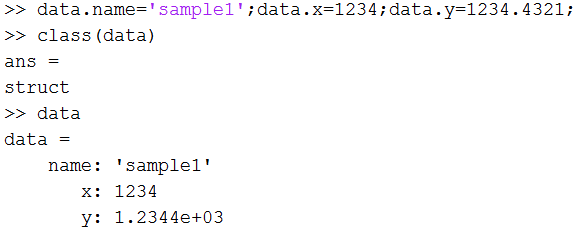
\includegraphics[scale=0.7]{structure_example}		
		\item It may be useful to know about these - see MATLAB Help for further reading
	\end{itemize}
\end{frame}

\section{Scripts}
\begin{frame}{Scripts}
	\begin{itemize}
		\item Enter edit at the prompt to start the Editor
		\item Or click on Home $\rightarrow$ New Script
		
		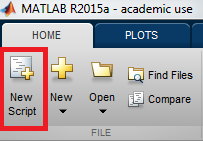
\includegraphics[scale=0.7]{new_script}	
		
		\item We can use the editor to write scripts (and also functions)
		\item It is much more powerful than entering commands at the prompt
		\item Advantages of scripts
			\begin{itemize}
				\item Easier for complex calculations
				\item Scripts can be edited and reused
				\item Calculations can be repeated
			\end{itemize}
	\end{itemize}
\end{frame}

\begin{frame}{Script files}
	\begin{itemize}
		\item Commands can be typed in a script and run as a program: type the list of commands into the editor instead of into the command window
		\item Typically each command is on a separate line
		\item Save to a file with .m extension, e.g. myscript.m
		
		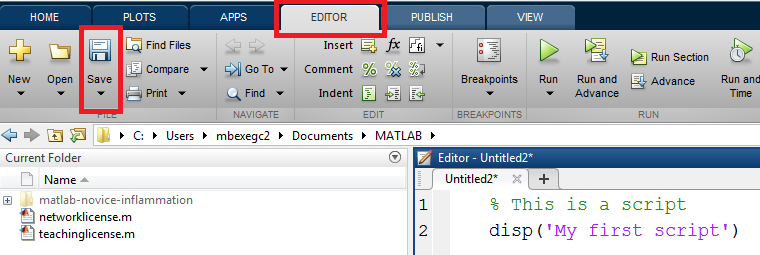
\includegraphics[width=0.9\textwidth]{save_script}
		\item Ensure script is in a directory on the MATLAB path (see slide \ref{sec:path} and \texttt{help path} for more info on the MATLAB path)
		\item Run the script by entering the name of the file (without the .m file xextension) e.g. myscript
	\end{itemize}
\end{frame}

\begin{frame}{Continuation of long lines}
	\begin{itemize}
		\item Use ... (three dots) to continue a command onto the next line so that it fits nicely into the editor
		
		
		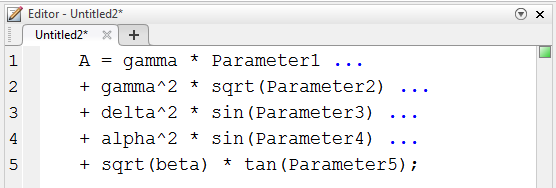
\includegraphics[scale=0.7]{editor_line_continuation}
	\end{itemize}
\end{frame}

\begin{frame}{Comments}
	\begin{itemize}
		\item Any text following \% is a comment
		\begin{itemize}
			\item Comments are ignored when the script is executed
			\item Comments can be used to explain how your code works
			\item Advice: add verbose comments so you understand everything your script does when you come to look at it later
		\end{itemize}
		\item The first comment line (referred to as the H1 line) is used by \texttt{lookfor} (\texttt{lookfor} searches for strings in the H1 line of \texttt{.m} files - see \texttt{help lookfor})
		\item The text in the first block of comments is returned by help (see \texttt{doc help }or \texttt{help help }for more info)
		\item It is good practice to write scripts that work with MATLAB’s help
		
		
	\end{itemize}
\end{frame}

\begin{frame}{Example script}{Used with \texttt{help }and \texttt{lookfor}}
	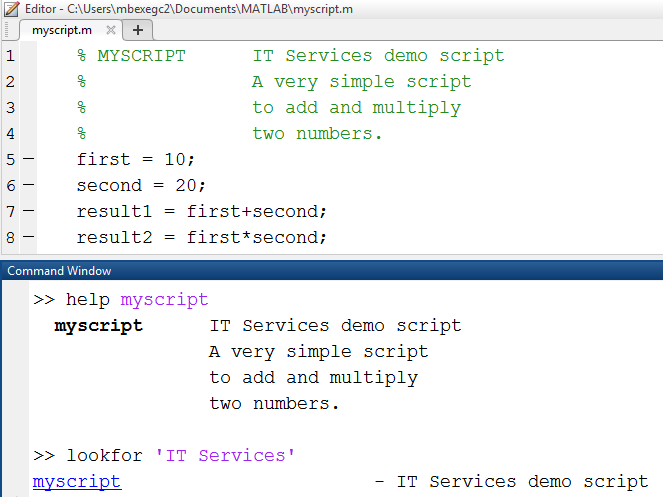
\includegraphics[width=0.85\textwidth]{script_help_lookfor}
\end{frame}

\begin{frame}{Using scripts}
	\begin{itemize}
		\item Scripts can call other scripts - \texttt{return} can be used to pass control back to the calling script or the keyboard
		\item Scope of variables
		\begin{itemize}
			\item A script has full access to all variables in the MATLAB workspace and in any calling script
			\item Variables created in a script persist after the script completes
			\item Therefore if using multiple scripts care must be taken when choosing variable names
			\item \textbf{For this reason, use of scripts is best reserved for simple tasks}	
			\item Write your own functions for more complex programming
		\end{itemize}
	\end{itemize}
\end{frame}

\frame{\frametitle{Good programming practice}
	\begin{itemize}
		\item Document your scripts and functions, so that you (or anyone else using your code) can understand how everything works
		
		\item When writing comments, assume you'll come back to the code in many years' time and won't remember anything about how it works
		\item Use variable names that describe what they are for
		\item Divide longer programs into logical units (e.g. using functions)
		
		Functions not covered in this course (look for examples in the MATLAB documentation, and consider attending the \href{https://app.manchester.ac.uk/rmatlabpro}{Programming in MATLAB} course)
	\end{itemize}
}

\subsection{Debugging scripts}
\frame{\frametitle{Tools for checking code}
	\begin{itemize}
		\item MATLAB has tools to report potential errors and improvements to your scripts e.g.
		\begin{itemize}
			\item Syntax errors e.g. missing brackets (these can be hard to spot in long m-files)
			\item Possible efficiency improvements
		\end{itemize}
		\item There are various interfaces to these tools
		\begin{itemize}
			\item MATLAB editor
			
			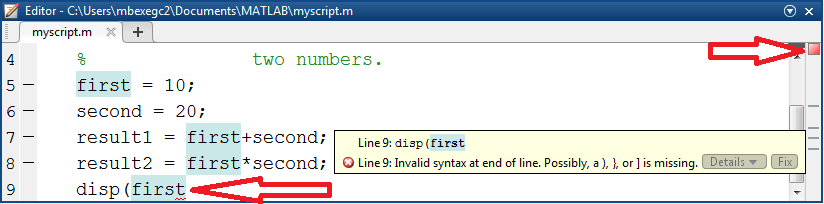
\includegraphics[width=0.9\textwidth]{editor_code_checking_tools}
			\begin{itemize}
				\item Underlines suspect code and gives helpful messages
				\item Provides coloured box to top right of window (red means potential problems)
			\end{itemize}
			
			
			\item \emph{Home} tab (code section) $\rightarrow$ \emph{Analyze Code}
			\item Check documentation for additional methods
		\end{itemize}  
	\end{itemize}
}

\frame{\frametitle{Debugging}
	\begin{itemize}
		\item MATLAB has very good \texttt{errors} and \texttt{warnings}
		\begin{itemize}
			\item These can help identify bugs
			\item We can also add \texttt{error} and \texttt{warning} messages to our code
		\end{itemize}
		\item We can also debug by outputting variable names
		
		e.g. use \texttt{fprintf}, \texttt{disp} or remove semicolons (see examples on next slide)
		\item MATLAB also has a very nice debugger
	\end{itemize}
}

\frame{\frametitle{Printing text to screen or files}
	\begin{itemize}
		\item \texttt{disp} displays single values or strings
		
		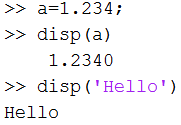
\includegraphics[scale=0.7]{disp}
		
		\item \texttt{fprintf} can print formatted text to screen (see \texttt{doc fprintf})
		
		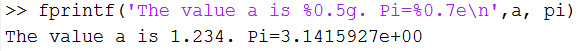
\includegraphics[scale=0.7]{fprintf}
		
		\item \texttt{fprintf} can also print formatted text to files
		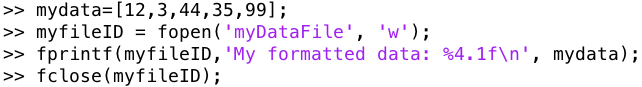
\includegraphics[width=\textwidth]{fprintf_file}

	\end{itemize}
}


\frame{\frametitle{The debugger}
	\begin{itemize}
		\item You can run the debugger from the MATLAB Editor (or from the prompt e.g. use \texttt{dbstop} function)
		\item Using the debugger we can
		\begin{itemize}
			\item Set stop points (including conditional stop points)
			\item Execute a program line by line, either stepping into or over functions
			\item View variables (three methods, all shown in screenshot below)			\begin{itemize}
				\item Hold the mouse cursor over a variable in the Editor
				\item Use the prompt (note the different prompt K$>>$)
				\item Use the Workspace window
			\end{itemize}
			
			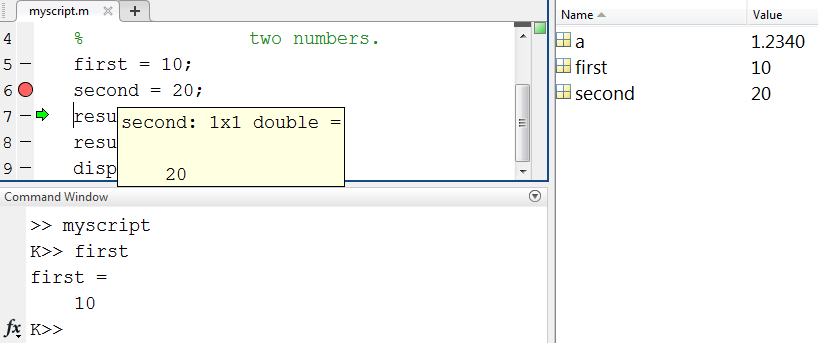
\includegraphics[width=0.7\textwidth]{debug}
		\end{itemize}
		
	\end{itemize}
}

\section{Arrays}
\frame{\frametitle{Arrays}
	\begin{itemize}
		\item An array is a systematic collection of data items
		\begin{itemize}
			\item In general arrays can have 1 or more dimensions
			\item Data in an array can be selected by indices (e.g. one index per dimension)
		\end{itemize}
		\item MATLAB arrays
		\begin{itemize}
			\item 2 or more dimensions
			\item Indexing starts at 1
			\item Arrays with zero size are allowed
			\item Arrays are dense by default (all values are stored in memory, even if they are zero)
			\item Sparse arrays are also available (only non-zero values are stored)
		\end{itemize}
		\item Note: arrays are different from the \texttt{cell} and \texttt{struct} classes
		\item Example of a 4$\times$6 array:
	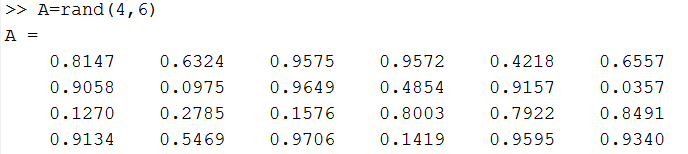
\includegraphics[width=\textwidth]{rand_array}
	\end{itemize}
}

\frame{\frametitle{Types of array}
	\begin{itemize}
		\item ALL MATLAB data is held in arrays
		\begin{itemize}
			\item Scalars: a special case of 2D array (size = 1$\times$1)
			\item Vectors: special case of 2D array (size 1$\times$n or n$\times$1, where n$>$1)
			\item Matrices: 2D arrays (size m$\times$n, where m$>$1 and n$>$1)
		\end{itemize}
		\item  Advised further reading for the mathematically inclined: Scalar, vector and matrix arithmetic
	\end{itemize}
}


\frame{\frametitle{Creating arrays}
	\begin{itemize}
		\item Use square brackets with semicolon to separate rows
		
		e.g. $>>$ A=[1 2; 3 4]
		\item Space (or comma) separates values in the same row
		\item Can create arrays from scalars or arrays (since scalars are considered 1$\times$1 arrays)
		
		e.g. $>>$ [A,A;A,A]
		\item Alternatively use MATLAB array generation functions, e.g. zeros, ones, rand, randn, eye
		
		e.g. $>>$ B=[A; rand(2,2); ones(2,2)];
		\item Zero length arrays are allowed, e.g. a=[]
		\item Try the examples given above
	\end{itemize}
}
\subsection{Accessing individual array elements}
\begin{frame}{Accessing individual array elements}{One index per dimension}
	\begin{itemize}
		\item Use parentheses and indices
		
		e.g. Y(3,4) for element at row 3, column 4 in 2D array Y
		\item Can access array elements on left or right of assignment operator
		
		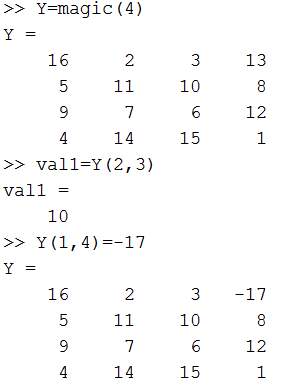
\includegraphics[width=0.4\textwidth]{array_access_pair_indices}	
		
	\end{itemize}
\end{frame}

\begin{frame}{Accessing individual array elements}{Single index notation}
	\begin{itemize}
		\item MATLAB stores elements contiguously in memory using column-wise ordering, i.e. array values are stored one after the other, a column at a time
		\item A single index can be used to access elements based on the column-wise ordering e.g.
		
		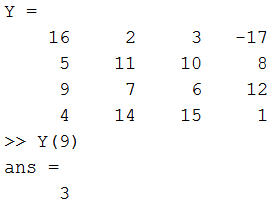
\includegraphics[width=0.5\textwidth]{array_access_columnwise}
		
		\item Enter \texttt{ help paren} for more information
	\end{itemize}
\end{frame}

\subsection{Accessing multiple array elements}
\begin{frame}{Accessing multiple array elements}
	\begin{itemize}
		\item Arrays can be used to index arrays e.g.
		
		X([4,2,5]) accesses elements with indices 4, 2 and 5
		(Reminder: create arrays using square brackets [ ])
		
		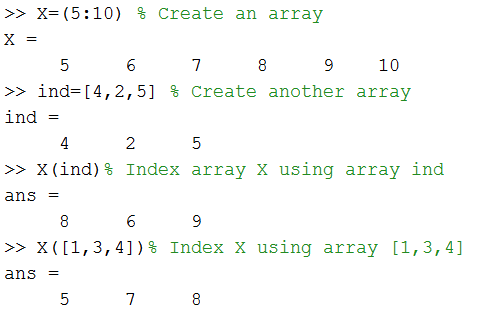
\includegraphics[scale=0.6]{array_access_array_index}
		
		\item We can use this to assign multiple values simultaneously e.g.
		
		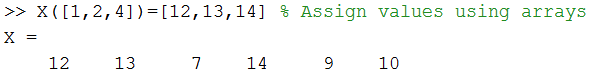
\includegraphics[scale=0.6]{array_assign_array_index}
	\end{itemize}
\end{frame}

%\subsection{Colon notation}
\begin{frame}{Accessing elements using colon notation}{Syntax}
	\begin{itemize}
		\item This creates vectors using \texttt{start}, \texttt{step} and end \texttt{values}
		\item The notation is \texttt{start:step:end}

		\texttt{step} is optional and defaults to 1
		
		\texttt{3:8} is equivalent to \texttt{3 4 5 6 7 8}
		
		\texttt{25:-2:20} is equivalent to \texttt{25 23 21}
		\item Enter \texttt{help colon} for more information
		\item We can use this notation to access multiple array elements
	\end{itemize}
\end{frame}

\begin{frame}{Accessing elements using colon notation}{Some examples}
	\begin{itemize}
		\item Colon notation allows us to access several elements at once 
		\item Try these examples for yourself, removing the semicolons to show the results
	\end{itemize}
	
	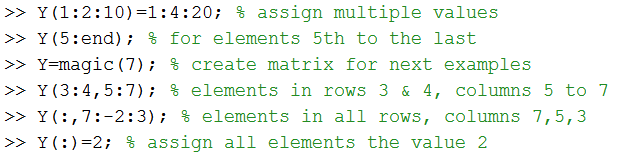
\includegraphics[scale=0.7]{colon_notation_array_examples}
\end{frame}

\subsection{Some useful array functions}
\begin{frame}{Some useful array functions}
	\begin{itemize}
		\item To find array size
		
		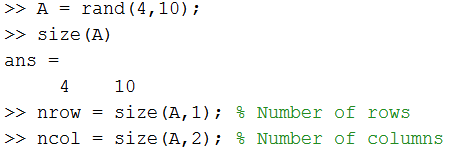
\includegraphics[scale=0.7]{array_size}
		
		\item To find number of dimensions
		
		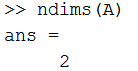
\includegraphics[scale=0.7]{array_ndims}
	\end{itemize}
\end{frame}

\subsection{Memory allocation}
\begin{frame}{Memory allocation - Preallocate arrays whenever possible!}{}
	\begin{itemize}
		\item Array memory allocation is automatic
		\begin{itemize}
			\item Arrays are extended as and when required
			\item Undefined values are filled with zeros
			\item Both are shown in the example below
		\end{itemize}
		
		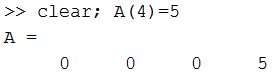
\includegraphics[scale=0.7]{array_memory_allocation}
		
		\item Extending arrays may be relatively slow
		\begin{itemize}
			\item e.g. growing a vector by 1 element each time a value is inserted.
			\item The entire array must be stored contiguously, so it may be necessary to copy
			all values to a new memory location each time the vector is extended.
		\end{itemize}

		\item Advice: \textbf{preallocate arrays whenever possible}
		\begin{itemize}
			\item i.e. create the array before using it
			\item e.g. use \texttt{zeros} function to create the array, then insert the values
		\end{itemize}
	\end{itemize}
\end{frame}

\subsection{Array operations}
\begin{frame}{Array operations}{}
	\begin{itemize}
		\item MATLAB (\textbf{MAT}rix \textbf{LAB}oratory) is designed to operate on matrices and arrays
		\item MATLAB functions will work with arrays, e.g.
		
		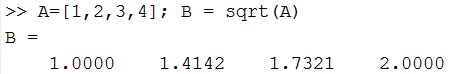
\includegraphics[scale=0.7]{array_operations_sqrt}
		
		\item Operators also work on arrays
		
		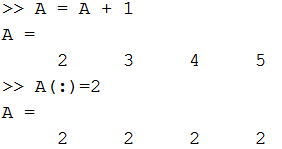
\includegraphics[scale=0.7]{array_operators}
	\end{itemize}
\end{frame}

\subsection{Matrix operators}
\begin{frame}{Matrix operators}{Syntax}
	\label{sec:matrix_operators}
	\begin{itemize}
		\item Some operators have two versions
		\begin{enumerate}
			\item Array operator\\
			Operates on individual elements (of same size arrays)
			\item Matrix operator\\
			Used to perform matrix operations
		\end{enumerate}
		\item . (dot) is used to differentiate the array operator if \textbf{(and only if)} there are 2 versions\\
		\item e.g. matrix multiply * versus array multiply .* (i.e. dot *)\\
		\texttt{A*B} multiplies matrix A by matrix B\\
		\texttt{A.*B} multiplies individual elements of arrays A and B\\
		\item e.g. matrix power \ $\hat{}$ \ versus array power .$\hat{}$\\
		\texttt{$A \ \hat{} \ 2$} is equivalent to \texttt{A*A} i.e. matrix power\\
		\texttt{$A \ . \hat{} \ 2$} calculates the square of each element in array A\\
	\end{itemize}
\end{frame}

\begin{frame}{Matrix operators}{Examples}
	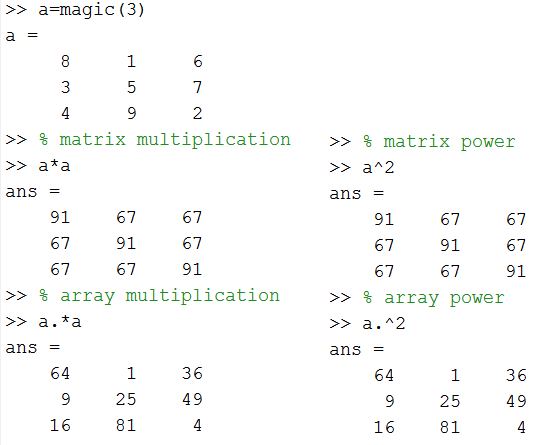
\includegraphics[width=\textheight]{matrix_array_operator_examples}
\end{frame}
	
\subsection{Plotting arrays}
\begin{frame}{Plotting arrays}{}
	\begin{itemize}
		\item MATLAB's plotting functions operate on arrays\\
		For example to plot sine between $-\pi$ and $\pi$
		
		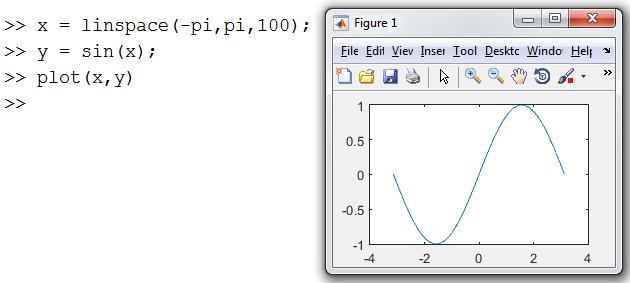
\includegraphics[width=\textwidth]{sine_plot}
		\item \texttt{linspace(x,y,n)} creates n equally spaced values from x to y
		\item For more on plotting
			\begin{itemize}
				\item Search \texttt{MATLAB Help} for \texttt{Plotting Basics}
				\item \url{http://uk.mathworks.com/discovery/gallery.html}
			\end{itemize}
	\end{itemize}
\end{frame}

\subsection{Sparse arrays}
\begin{frame}{Sparse arrays}{}
	\begin{itemize}
		\item These only store non-zero values in memory
		\item Some calculation generate large matrices containing few non-zero values\\
		e.g. finite element modelling
		\item It would be very inefficient to store and use all the zero values
		\item It would also limit the largest problem size which could be stored in memory
		\item Hence it may be useful to know about sparse arrays
	\end{itemize}
\end{frame}

\section{Finding help}
\begin{frame}{Finding help}
	\begin{itemize}
		\item MATLAB has very good documentation (see slide \ref{sec:matlab_help}), which contains  example code snippets. Copying and pasting example code at the prompt is a good way to learn about new features.
		\item There are tutorials contained within the MATLAB documentation\\		
		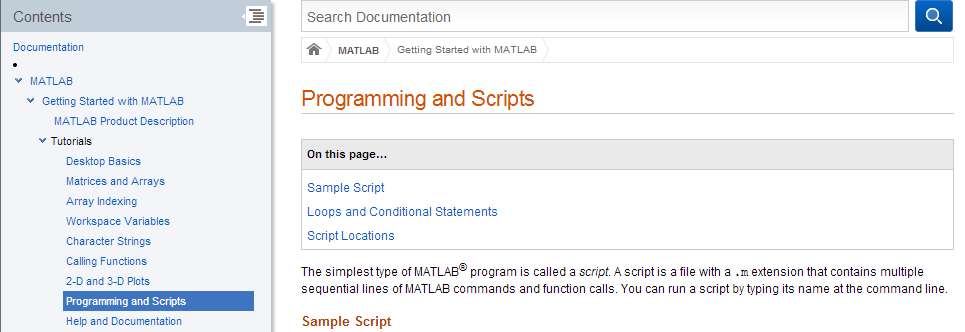
\includegraphics[width=\textwidth]{matlab_doc_tutorials}
		\item \href{http://uk.mathworks.com/matlabcentral/?s_tid=gn_mlc}{MATLAB central} is a user forum where you can find the answers to many MATLAB questions
		\item Search on google
	\end{itemize}
\end{frame}

\end{document}
